%% Digital Systems
%% Continuous System Equivalence
\def\FileDate{10/01/21}
\def\FileVersion{1.0}
% ----------------------------------------------------------------
% Notes pages *********************************************************
% ----------------------------------------------------------------

\begin{slide}
	\heading{Purpose of this Lecture}
	To describe the basic tools for the design of a control system to be implemented using a computer or microcomputer.

	\textbf{Contents}
	\begin{itemize}
		\item Typical architecture
		\item Relationship between $s$ and $z$
		\item Continuous design followed by Discretization
		\item Direct digital design
	\end{itemize}
\end{slide}

\section*{Typical Architecture of a Digital Control System}

\begin{slide}
	\heading{Typical Architecture}
	\begin{center}
	\resizebox{300pt}{!}{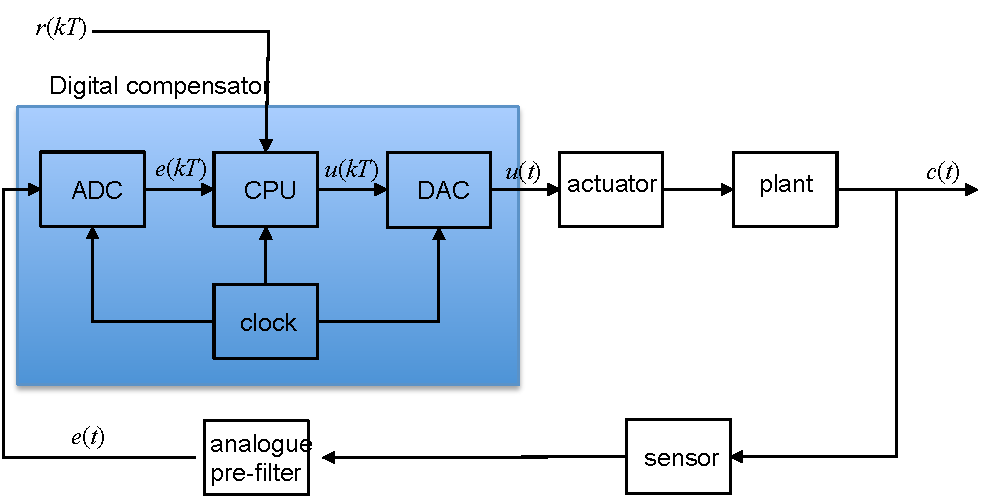
\includegraphics{pictures/digicon.pdf}}
\end{center}
\end{slide}

\section*{Relationship between $s$ and $z$}

We have already seen (SLIDE~2, lecture 12) that
\ifslidesonly
\begin{slide}
\heading{Relationship between $s$ and $z$}
We have already seen (see last lecture) that
\begin{equation}\label{eq:l12e1a}
	z=e^{sT}
\end{equation}
and
\begin{equation}\label{eq:l12e1b}
	s=\frac{1}{T}\ln z
\end{equation}
\endinput

\end{slide}
\fi
\begin{equation}\label{eq:l12e1a}
	z=e^{sT}
\end{equation}
and
\begin{equation}\label{eq:l12e1b}
	s=\frac{1}{T}\ln z
\end{equation}
\endinput


We can use Equation~\ref{eq:l12e1a} to define a mapping between the $s$ and $z$ planes as summarised in SLIDES~\ref{slide:l12s2} and \sref{slide:l12s3}.
\begin{slide}\label{slide:l12s2}
  \heading{Mapping between between $s$ and $z$}
  Since $z=e^{sT}$ we can define a `mapping' from the $s$-plane to the $z$-plane. Various properties of the $z$-plane follow.
\begin{itemize}
  \item s-plane stability boundary $s=j\omega$ maps to the unit circle $|z|=1$ in the z-plane.
  \item Maximum frequency is half the sampling frequency $\omega_s/2$ (a consequence of Nyquist's sampling theorem) and is mapped to the negative real axis in the z-plane.
\end{itemize}
For proofs, see the problems in the self-directed learning exercises.
\end{slide}

\begin{slide}\label{slide:l12s3}
  \heading{Stability in the z-plane}
\begin{itemize}
  \item Because the stability boundary is a unit circle, Routh-Hurwitz and Nyquist stability tests no longer work.
  \item The Jury test is a similar test to the Routh-Hurwitz test but it is more involved.
  \item The design curves for constant natural frequency $\omega_n$, damping ratio $\zeta$, $\sigma_d$ and $\omega_d$ are also distorted by the mapping.
  \item Use the Matlab function \emph{zgrid} to see the mapping.
\end{itemize}
\end{slide}

\begin{slide}\label{slide:l12s4}
  \heading{z-plane Design Curves}
  \begin{center}
    \scalebox{0.3}{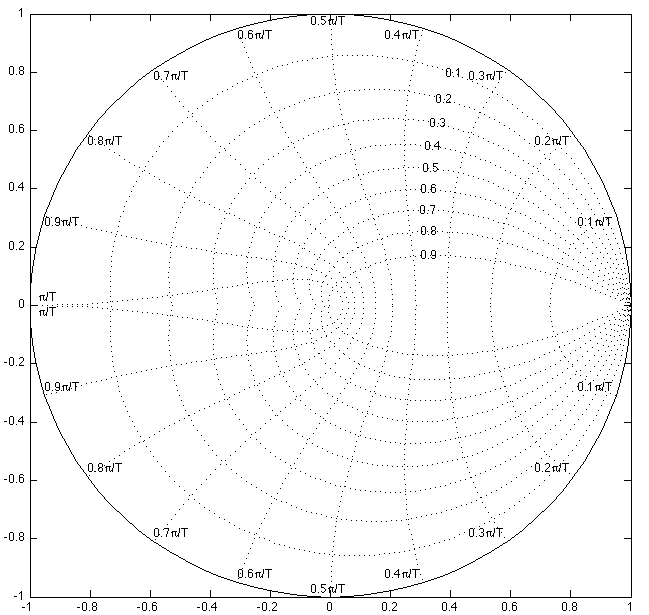
\includegraphics{pictures/zgrid.png}}
  \end{center}
\end{slide}


\section*{Continuous Design}

Assumption -- we have designed a compensator using root-locus or frequency response and now need to implement it with digital hardware, e.g. a digital micro-controller or digital signal processor (DSP).

We will recall the Discretization methods discussed in the last lecture, give a comparison of their frequency response behaviour and the applicability of the continuous design approach. We conclude with an example.

\subsection*{Discretization Procedure}

The idea is that given a continuous compensator transfer function $D(s)$ we need to find the best equivalent $D(z)$. As illustrated in \sref{slides:l12s6}, there is no exact solution since the whole time history is available to $D(s)$ whereas only samples are available to $D(z)$ so different discretization approximation methods make different assumptions about what happens to $e(t)$ between sampling instants.

\begin{slide}\label{slides:l12s6}
	\heading{Discretization Procedure}
	Given a continuous $D(s)$ find best equivalent $D(z)$.
	\begin{center}
		\resizebox{200pt}{!}{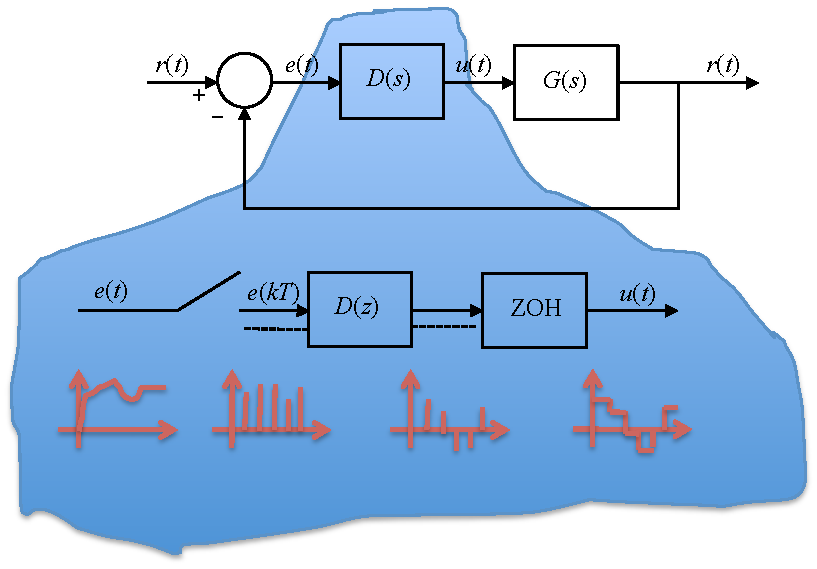
\includegraphics{pictures/digitization.pdf}}
	\end{center}
\end{slide}

\begin{slide}
	\heading{Discretization with Matlab}
	Take a transfer function (here $D(s)=p/(s+p)$) and return an equivalent $D(z)$
\begin{verbatim}
p = 5; % rad/s
ds = tf([p], [1 p])
Fs = (20*p)/(2*pi); % Hz
Ts = 1/Fs;
dz = c2d(ds, Ts, method)
step(ds,'-',dz,'--')
\end{verbatim}
\end{slide}

\begin{slide}
	\heading{Summary of Discretization Methods}
	See Lecture 11 for mathematical derivations.
	\begin{center}
		\begin{tabular}{|l|l|l|}
			\hline
			\textbf{Method} & \textbf{Transform} & \textbf{c2d method} \\
			\hline
			Zero-order hold & $(1-z^{-1})\mathcal{Z}(D(s)/s)$ & \verb|'zoh'| \\
			\hline
			Tustin (bilinear transform) & $s = (2/T)(1-z^{-1})/(1+z^{-1})$ & \verb|'tustin'| \\
			\hline
			Matched pole-zero & map poles/zeros using $z=e^{sT}$ & \verb|'matched'| \\
			\hline
			First-order hold & See Matlab documentation & \verb|'foh'| \\
			\hline
			Impulse-invariant & See Matlab documentation & \verb|'imp'| \\
			\hline
			Tustin with pre-warp & See Matlab documentation & \verb|'prewarp'| \\
			\hline
		\end{tabular}
	\end{center}
\end{slide}

\subsection*{Comparison of approximations}

\ifslidesonly
\begin{slide}
\heading{Comparison of approximations}
Run script \emph{comparison.m} that you will find on Blackboard.
\end{slide}
\fi
Run script \emph{comparison.m} that you will find on Blackboard.
You should note that the approximations are good for frequencies below about $\omega_s/4$.
If $\omega_s$ is sufficiently high, then break frequencies are accurately reproduced.
MPZ and Tustin show a notch at $\omega_s/2$ because of the zero term at $1+z^{-1}$.
Apart from the large difference at $\omega_s/2$, which is typically outside the
working frequency, all methods have similar performance. Since MPZ is easier to
calculate by hand, it is often to be preferred. However, if you have access to
Matlab and the control system toolbox function \emph{c2d}, there is no need to
use anything other than ZOH (which is the default) or the Tustin method.

\ifslidesonly
\begin{slide}
\heading{Plan for the live session}
In the session we will:
\begin{itemize}
\item design a continous compensator for a plant and discretize it by MPZ method
\item see how the digital compensator would be implemented
\item discuss the limitations of "continuous design"
\item redesign the compensator using a digital-design approach.
\end{itemize}
\end{slide}
\fi

\begin{slide}
	\heading{Design Example}\label{slides:ex1-1}
	\resizebox{300pt}{!}{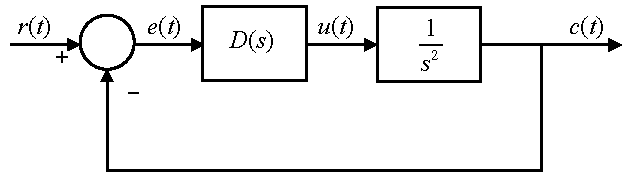
\includegraphics{pictures/ex1-1.pdf}}
\end{slide}


\subsection*{Design Example}

Let us consider the lead compensation of the double integrator system shown in \sref{slides:ex1-1}. Let us further assume that we want to have the dominant closed-loop poles with ideal damping $\zeta=1/\sqrt{2}$ and natural frequency $\omega_n = 2\sqrt{2}$ rad/s. Furthermore, let us assume that the zero will be placed at $s=-1$ so that the compensator $D(s) = K(s+1)/(s+p)$. The root-locus design parameters will then be obtained from the pole-zero map shown in \sref{slides:ex1-2}.

$$\theta_z = \tan^{-1} 2/1 = 116.57^\circ$$

\begin{eqnarray*}
	-\theta_p + 116.57 -270 & = & -180 \\
	-\theta_p & = & -180 - 153.43 \\
	\theta_p & = & 26.57^\circ
\end{eqnarray*}

\begin{eqnarray*}
	-\tan 26.57 & = & \frac{2}{x} \\
	x & = & 2/\tan 26.57 = 4 \\
	p & = & -6
\end{eqnarray*}


\begin{slide}\label{slides:ex1-2}
	\heading{Root Locus Design Parameters}
	\resizebox{300pt}{!}{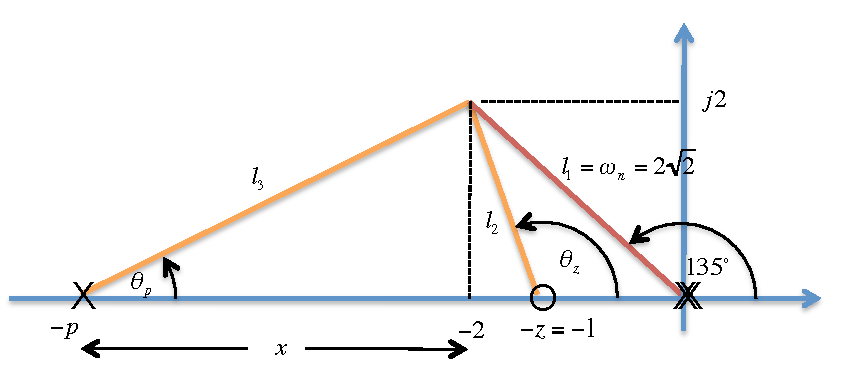
\includegraphics{pictures/ex1-2.pdf}}
\end{slide}

To calculate the gain, we need to know that $l_1=2\sqrt{2}$, $l_2=\sqrt{5}$, $l_3=\sqrt{20}$.

$$K = \frac{(2\sqrt{2})^2\times \sqrt{20}}{\sqrt{5}} = \frac{8\times 2\sqrt{5}}{\sqrt{5}} = 16.$$

$$D(s) = \frac{16(s+1)}{(s+6)}.$$

To convert to $D(z)$ let the sampling frequency $\omega_s=20\times \omega_n = 40\sqrt{2}=56.67$ rad/s. Thus $f_s=\omega_s/2\pi = 9$~Hz so sampling period $T = 1/f_s \approx 0.1$~s.

Let's pretend that we are solving this problem in a context where we only have a calculator so we'll use matched-pole zero.

$$D(z)=k\frac{1-e^{-aT}z^{-1}}{1-e^{-bT}z^{-1}}$$

where $k$ is determined by matching the DC gain of the two compensators. For the continuous compensator $D(s)|_{s=0} = 16/6$. For the digital compensator $D(z)|_{z=1} = k(1-e^{-aT})/(1-e^{-bT})$, so

$$k=\frac{16}{6}\times\frac{1-e^{-bT}}{1-e^{-aT}}$$

For our design, $T=0.1$, $a=1$ and $b=6$ so
\begin{eqnarray*}
	k & = & \frac{16}{6}\times\frac{1-e^{-0.6}}{1-e^{-0.1}} \\
	&= & \frac{16}{6}\times\frac{1-0.5488}{1-0.9048} = \frac{16}{6}\times\frac{0.4512}{0.0952}  \\
	k & = & 12.64
\end{eqnarray*}

So $$D(z) = \frac{12.64(1-0.9048z^{-1})}{(1-0.5488z^{-1})}$$

\ifslidesonly
\begin{slide}
\heading{Implementation of design}
The simplest converter is a ``\emph{Zero-Order Hold}'' (see
Fig.~\ref{fig:l11f1}). This acts the opposite way to a sampler.
\begin{figure}[htbp]
  \begin{center}
    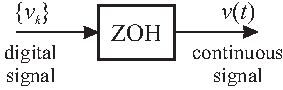
\includegraphics{pictures/zoh.pdf}
    \caption{Zero-Order Hold}
    \label{fig:l11f1}
  \end{center}
\end{figure}
\endinput

\end{slide}
\fi
The simplest converter is a ``\emph{Zero-Order Hold}'' (see
Fig.~\ref{fig:l11f1}). This acts the opposite way to a sampler.
\begin{figure}[htbp]
  \begin{center}
    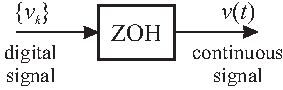
\includegraphics{pictures/zoh.pdf}
    \caption{Zero-Order Hold}
    \label{fig:l11f1}
  \end{center}
\end{figure}
\endinput


\ifslidesonly
\begin{slide}
\heading{Implementation of design - pseudocode}
During each sample period, the device holds the output $v(t)$ constant
at the current value of the digital signal $v_k$. That is
\begin{equation}
  \label{eq:l11e4}
  v(t) = v_k\ \mathrm{for}\ kT \le t < (k+1)T
\end{equation}
This generates a stepwise continuous signal $v(t)$ which at the
sampling instants is equal to the continuous signal from which the
digital signal ${v_k}$ was generated (\sref{slide:l11s3}).
\endinput

\end{slide}
\fi
During each sample period, the device holds the output $v(t)$ constant
at the current value of the digital signal $v_k$. That is
\begin{equation}
  \label{eq:l11e4}
  v(t) = v_k\ \mathrm{for}\ kT \le t < (k+1)T
\end{equation}
This generates a stepwise continuous signal $v(t)$ which at the
sampling instants is equal to the continuous signal from which the
digital signal ${v_k}$ was generated (\sref{slide:l11s3}).
\endinput



\ifslidesonly
\begin{slide}
\heading{Limitations of Continuous Design Approach}
\begin{itemize}
\item Limitations on sampling rate
\item Lag effect of ZOH at low-sampling rates
\end{itemize}
See notes for more detail.
\end{slide}
\fi
\subsection*{Limits of Continuous Design Approach}

If an exact discrete analysis or a simulation of a system were performed and
discretization determined for a large range of sampling rates the digitised
system would be unstable for rates slower than approximately $5\omega_n$
(where $\omega_n$ is the natural frequency of the system dominant poles)
and damping would be degraded for rates slower than $10\omega_n$.
At sampling rates higher than $20\omega_n$ (or $20\times \omega_{BW}$ for
more complex systems) then all methods yield reasonable results and can be used
with confidence at rates of $30\times \omega_{BW}$ or higher.

Errors come about because the approximations ignore the phase lag effect of the
zero-order-hold (ZOH). The ZOH can be approximated by $$G_{zoh}(s)\approx
\frac{2/T}{s+(2/T)}$$ which is based on the idea that, on average, the ZOH delays
the signal by about $T/2$ seconds and this transfer function is a first-order
lag with time constant $T/2$ and DC gain of 1. If this was added to the plant
transfer function then a more accurate model of the delayed plant wiould be
obtained and a more stable design for $D(s)$.

However, the advantage of continuous design is that $T$ is not chosen until
after $D(s)$ is designed and the appearance of $T$ so early invalidates this
assumption.

\ifslidesonly
\begin{slide}
\heading{Direct Digital Design}
\begin{itemize}
\item Used when limitations on sampling would be breached.
\item Stability boundary is unit circle which adds complications not present for
continous time systems
\item Additional complexity added because of distorting effect of the mapping $z=e^{sT}$
\end{itemize}
We will illustrate with an example.
\end{slide}
\fi
\section*{Direct Digital Design}

Direct digital design may be used if the zero-order hold is to be taken into
account or if the sample time is somehow constrained. The discrete transfer
function for the plant, hold and compensator are used throughout and the root
locus method\footnote{Frequency response methods can be used, but are complicated
by the fact that the stability boundary is the unit circle. We leave the methods,
which are well covered in Franklin, Powell and Workman, as a topic for further
research.} is used in the $z$-domain.

In this presentation, we will consider how the plant is digitized and how the
compensator can be designed using the root locus technique in the $z$-domain.

\subsection*{Analysis Tools}

\begin{slide}\label{slides:l12s11}
	\heading{Assumed architecture}
	\resizebox{300pt}{!}{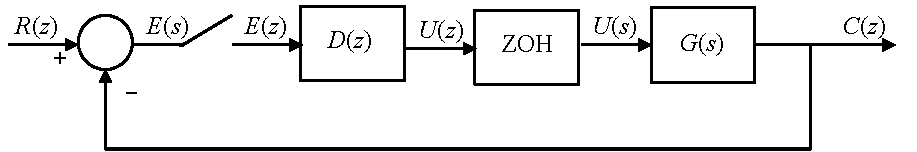
\includegraphics{pictures/digisys.pdf}}
\end{slide}

\begin{slide}\label{slides:l12s12}
	\heading{Discrete equivalent}
	\resizebox{300pt}{!}{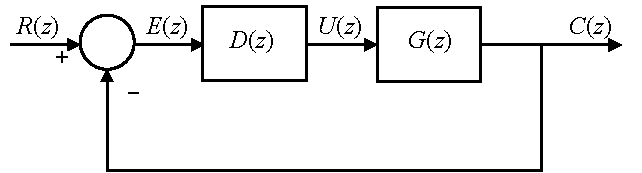
\includegraphics{pictures/digequiv.pdf}}
\end{slide}

The zero-order hold (ZOH) precisely defines what happens to the continuous system between samples for there is a unique solution for the combination of the transfer functions of the ZOH and G(s). The transfer function for ZOH  (see Lecture 11) is $(1-e^{-sT})/s$ so for hold followed by plant we can use the mathematical development show in \sref{slides:l12s13} to determine $G(z)$. As we showed in Lecture 11 (see SLIDE~4), the $1/s$ term is present because the output of ZOH is a piecewise constant function of time, and $1-z^{-1}$ represents a step followed by a negative step delayed by one sample period.


\begin{slide}\label{slides:l12s13}
	\heading{Hold Plus Plant}

	\begin{eqnarray*}
		\left(\frac{1-e^{-sT}}{s}\right)G(s) & = & (1-e^{-sT})\frac{G(s)}{s} \\
		\mathcal{Z}\left\{(1-e^{-sT})\frac{G(s)}{s}\right\} & = & \mathcal{Z}\{1-e^{-sT}\}\mathcal{Z}\left\{\frac{G(s)}{s}\right\} \\
		G(z) & = & (1-z^{-1}) \mathcal{Z}\left\{\frac{G(s)}{s}\right\}
	\end{eqnarray*}
\end{slide}

For the discrete equivalent system of \sref{slides:l12s12}

$$\frac{C(z)}{D(z)} = \frac{DG(z)}{1+DG(z)}$$ and the closed-loop characteristic equation (CLCE) is $$1+DG(z)=0.$$ The root-locus plotting rules still apply but the interpretation is different.

\subsubsection*{Example}

$$G(s)=\frac{a}{s+a}$$

\begin{eqnarray*}
	G(z) & = & (1-z^{-1})\mathcal{Z}\left\{\frac{a}{s(s+a)}\right\} \\
	     & = & (1-z^{-1})\mathcal{Z}\left\{\frac{1}{s}-\frac{1}{s+a}\right\} \\
	     & = & (1-z^{-1})\left\{\frac{z}{z-1}-\frac{z}{z+e^{-aT}}\right\} \\
		 & = & \left(\frac{z-1}{z}\right)\left\{\frac{z(z-e^{-aT})-z(z-1)}{(z-1)(z+e^{-aT})}\right\} \\
\end{eqnarray*}
$$G(z) = \frac{1-e^{-aT}}{z-e^{-aT}}.$$
So $G(z)=(1-\alpha)/(z-\alpha)$ where $\alpha=e^{-aT}$. The implications of this result is assessed in SLIDES~\ref{slides:l12s14} and \ref{slides:l12s15}.
\begin{slide}\label{slides:l12s14}
	\heading{Root locus of plant $G(s)=a/(s+a)$}
	\begin{center}
		\resizebox{220pt}{!}{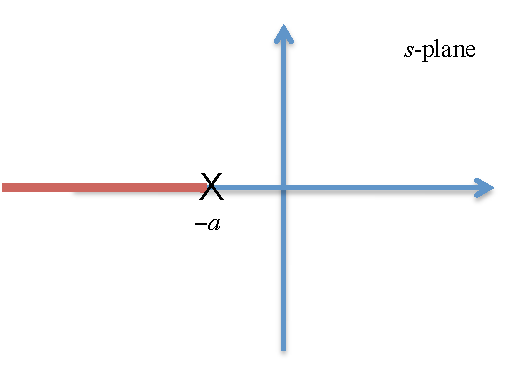
\includegraphics{pictures/slocus.pdf}}
	\end{center}
	This is stable for all open-loop gain $K$.
\end{slide}
\begin{slide}\label{slides:l12s15}
	\heading{Root locus of hold-equivalent plant $G(z)=(1-\alpha)/(z+\alpha)$}
	\begin{center}
		\resizebox{200pt}{!}{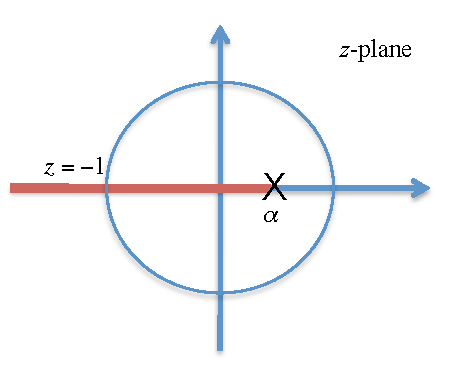
\includegraphics{pictures/zlocus.pdf}}
	\end{center}
	This is unstable for some gain $K$ because of the time delay introduced by ZOH.
\end{slide}

\begin{slide}\label{slides:l12s16}
	\heading{Discrete Three Term Compensators}
	\begin{tabular}{|l|l|l|}
	\hline
	\textbf{Type} & \textbf{Implementation} & \textbf{Transfer function} \\
	\hline
	Proportional & $u(n) = K_Pe(n)$ & $D(z)=K_P$ \\
	\hline
	Derivative & $u(n) = K_D(e(n)-e(n-1)$ & $D(z)=K_D(1-z^{-1})$ \\
	\hline
	Integral & $u(n) = u(n-1) + K_Ie(n)$ & $D(z)=K_I/(1-z^{-1})$\\
	\hline
	\end{tabular}
\end{slide}

Of course, these can be combined to give P+D and PID. There are also equivalents of lead, lag and lead-lag.

\subsection*{Design example repeated}

\begin{slide}\label{slides:l12s17}
	\heading{Example: Double-integrator plant again}
	$$G(s)=\frac{1}{s^2}$$
	Hold equivalent is
	$$G(z)=\frac{T^2}{2}\frac{(z+1)}{(z-1)^2}$$
	Let $T = 0.1$ seconds then
	$$G(z)=\frac{1}{200}\frac{(z+1)}{(z-1)^2}$$
\end{slide}

\begin{slide}\label{slides:l12s18}
	\heading{Root locus}
	\begin{center}
		\resizebox{200pt}{!}{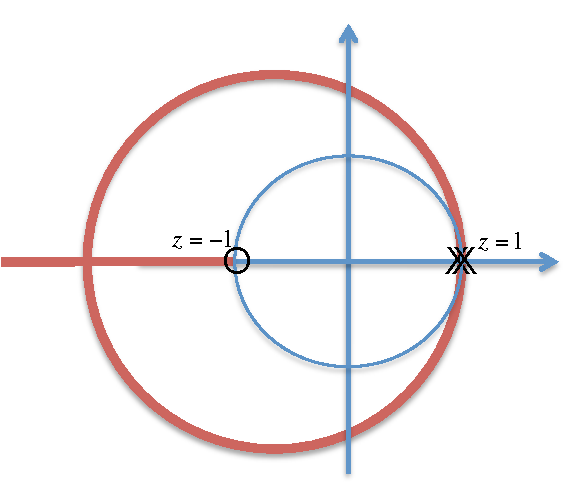
\includegraphics{pictures/zdi.pdf}}
	\end{center}
	Note, root-locus is outside unit circle so system is unstable for all $K_P$.
\end{slide}

We introduce proportional plus derivative compensation to bring the root locus inside the unit circle. Thus, from the table in \sref{slides:l12s16} $$U(z)=K_PE(z)+K_D(1-z^{-1})E(z)$$ Hence
\begin{eqnarray*}
	D(z) = \frac{U(z)}{E(z)} & = & K_P + K_D - K_D z^{-1} \\
	& = & \frac{(K_P+K_D)z - K_D}{z} \\
	& = & (K_P+K_D)\left(\frac{z-(K_D/(K_P+K_D))}{z}\right) \\
	& = & K_c\left(\frac{z-\gamma}{z}\right)
\end{eqnarray*}
We note that $$DG(z)=\frac{K_c}{200}\left(\frac{z-\gamma}{z}\right)\frac{(z+1)}{(z-1)^2}$$ and hence the root-locus gain $K_o=K_c/200$. The compensator adds a pole at $z=0$ and a zero at $z=\gamma$.

As before, we would like the system to have ideal damping and a natural frequency of $2\sqrt{2}$. But as we are now working in the $z$-plane, we also need to map the desired closed-loop poles by the mapping $s=e^{sT}$.

Since $s=-2\pm j2$ and $z=e^{sT}$ then $z=e^{-2T}e^{\pm j2T} = e^{-0.2}(\cos0.2\pm j\sin0.2) = 0.8024\pm j0.1627$. Given this location for the desired closed-loop dominant poles, it is a matter of trigonometry to determine that $\gamma=0.8532$ and the root locus gain $K_o=0.0465$. Now since $K_c=200 K_o = 9.31$ it is easy to show that $K_D=7.9367$ and $K_P=1.3703.$ The proof is left as an exercise.

%----------------------------------------------------------------
% The end of notes
% ----------------------------------------------------------------
\endinput

% Local Variables:
% TeX-master: "lecture03"
% End:
